\documentclass[12pt,a4paper]{article}
\usepackage[utf8]{inputenc}
\usepackage{graphicx}
\author{Abdelsalam ElTamawy, Sara Ahmed}
\title{4 Bit ALU Project}
\begin{document}

\maketitle


\pagebreak

\section{Contributions}
Both team members worked tirelessly to make this project a success. We started out by meeting up to brainstorm the circuit. We then ultimately decided that Abdelsalam would complete the schematic diagram, while Sara was to work on the block design. Both designs were done on Logisim. Once that was completed, and confirmed, Abdelsalam took it upon himself to buy the equipment for the project, and we met up to complete it on Wednesday the 27th, and Thursday the 28th.

\section{How to Use}
The furthest 4 switches on the left are dedicated to the first input(A). The furthest 4 switches on the right are dedicated to the second input(B). These orientations assume the side with the switches are closest to you. The set of 3 switches that are in the middle control which operational mode the circuit is in. These operational modes are defined as follows.

\begin{center}

\begin{tabular}{c|c|c||l}
$OP_1$ & $OP_2$ & $OP_3$ & \multicolumn{1}{|c}{mode} \\ 
\hline 
0 & 0 & 0 & AND \\ 
\hline 
1 & 0 & 0 & OR \\ 
\hline 
0 & 1 & 0 & XOR \\ 
\hline 
1 & 1 & 0 & NOR \\ 
\hline 
0 & 0 & 1 & Logical shift right A \\ 
\hline 
1 & 0 & 1 & Arithmetic shift right A \\ 
\hline 
0 & 1 & 1 & Rotate left B \\ 
\hline 
1 & 1 & 1 & Shift left A \\ 
\end{tabular}
\end{center}

\section{Block diagram}

\noindent\makebox[\textwidth]{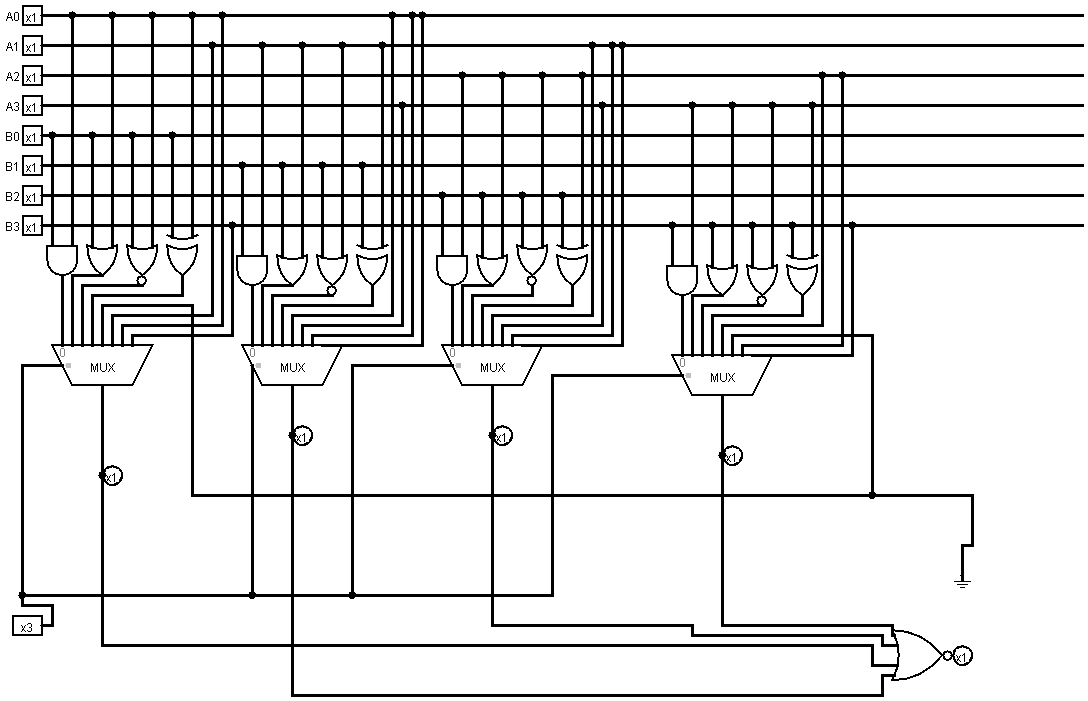
\includegraphics[width=\paperwidth]{block_diagaram.png}}


\section{Circuit diagram}

\noindent\makebox[\textwidth]{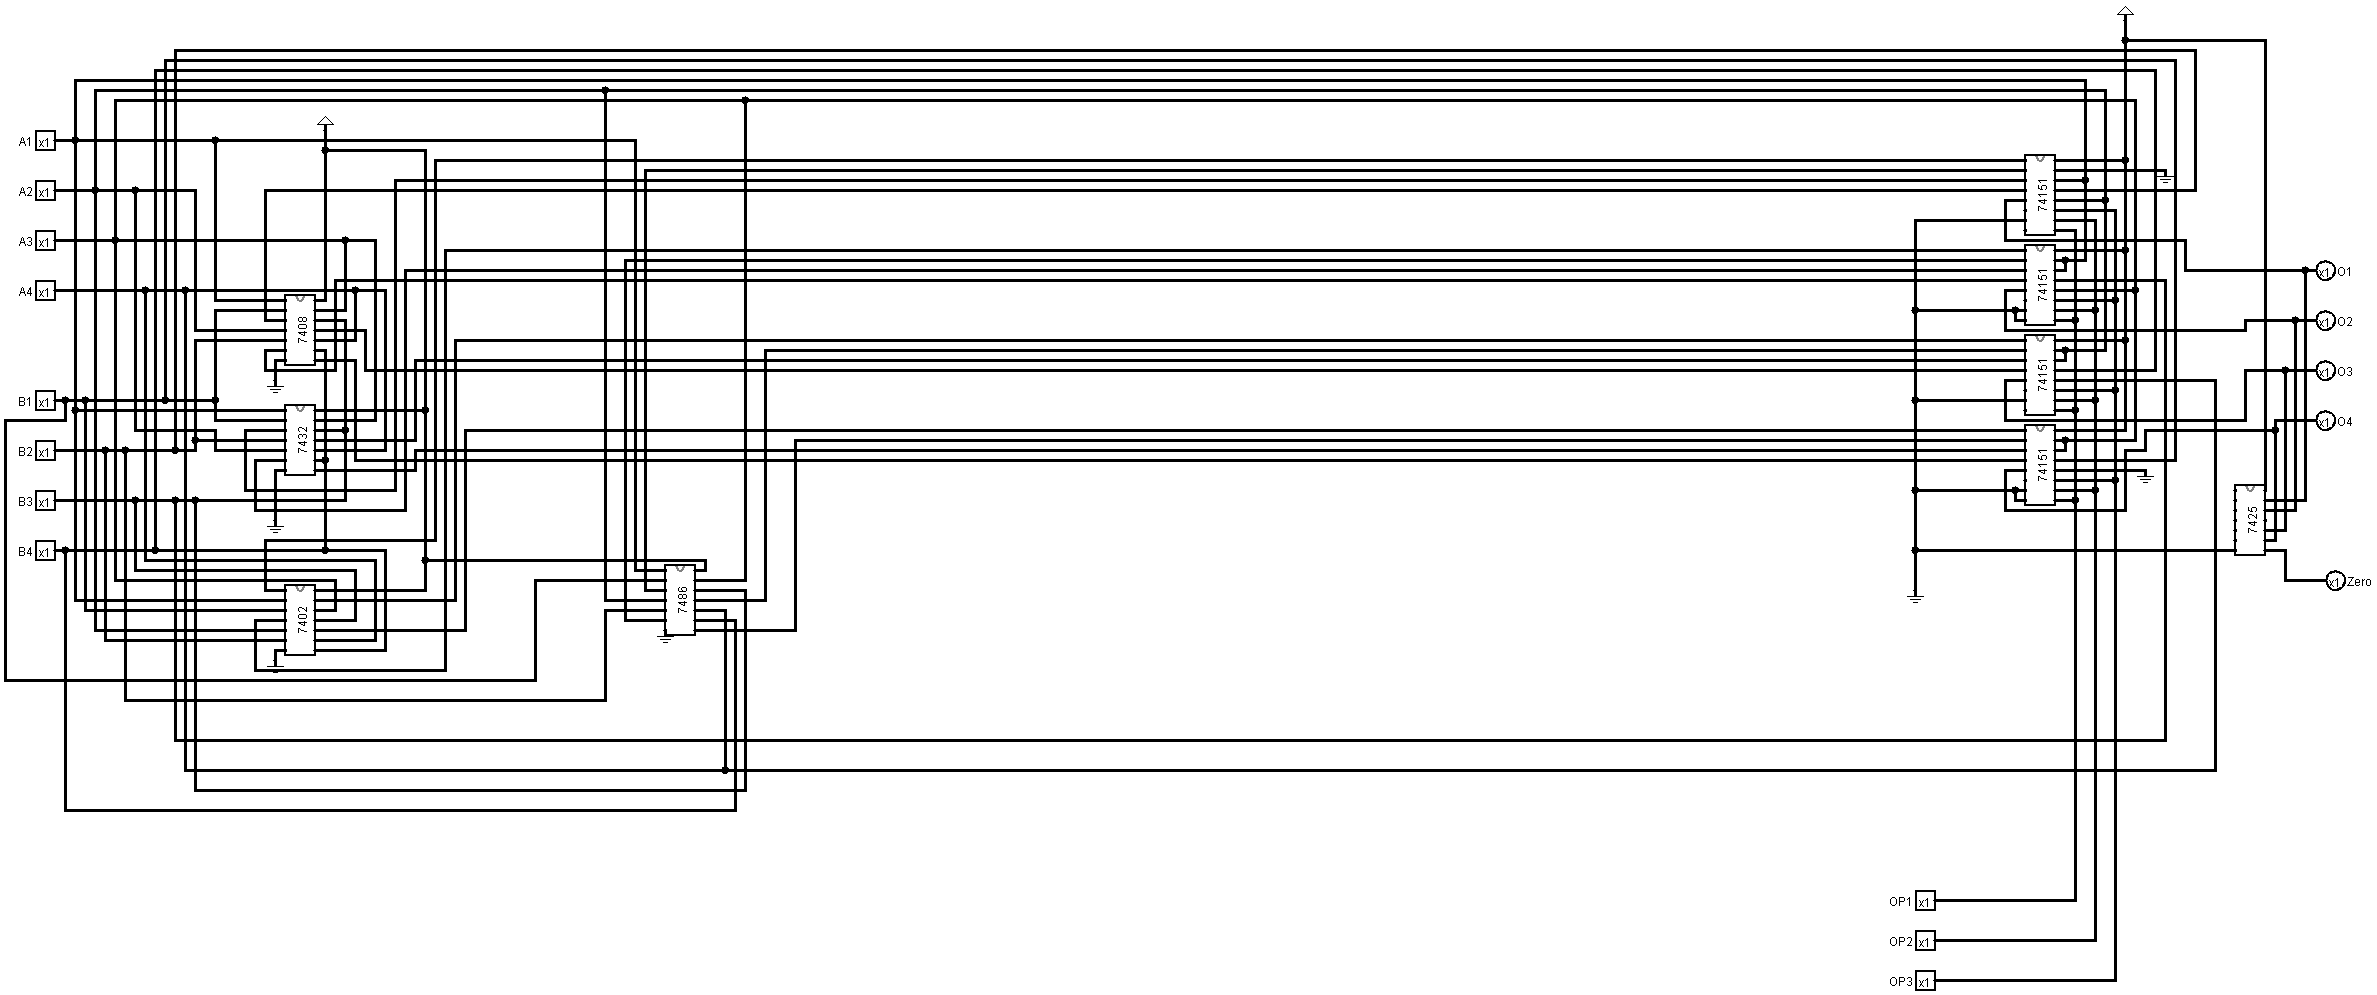
\includegraphics[width=\paperwidth]{curcuit_schematic.png}}


\end{document}